\documentclass[polish,envcountsect,10pt]{beamer}
\usetheme{metropolis}
\usepackage[T1]{fontenc}
\usepackage{polski}
\usepackage{babel}
\usepackage{tikz}
\usepackage{graphicx}
\usepackage{xcolor}
\graphicspath{ {./img/} }

\title{Triangulacja i diagramy Voronoi}
\author{Krzysztof Nasuta}
\date{Gdańsk, 2025}

\begin{document}

\frame{\titlepage}

% Triangulacja w geometrii

\begin{frame}
  \frametitle{Triangulacja w geometrii}
  \begin{definition}
    Sympleks to uogólnienie trójkąta i czworościanu na dowolne wymiary. Są to najprostsze możliwe obiekty geometryczne w danym wymiarze.
  \end{definition}

  \pause
  Dla przykładu:
  \begin{itemize}
    \item 0-wymiarowy sympleks to punkt,
    \item 1-wymiarowy sympleks to odcinek,
    \item 2-wymiarowy sympleks to trójkąt,
    \item 3-wymiarowy sympleks to czworościan,
  \end{itemize}
\end{frame}

\begin{frame}
  \frametitle{Triangulacja w geometrii}
  \begin{definition}
    Triangulacja to podział płaszczyzny euklidesowej na trójkąty. W ogólności mówi się o podziale przestrzeni euklidesowej na sympleksy odpowiedniego wymiaru.

    \pause
    Zazwyczaj wymagane jest, aby krawędzie i wierzchołki sympleksów pokrywały się w całości z krawędziami i wierzchołkami innych sympleksów.
  \end{definition}
\end{frame}

\begin{frame}
  \frametitle{Triangulacja w geometrii - przykład dwuwymiarowy}
  \begin{center}
    \begin{figure}
      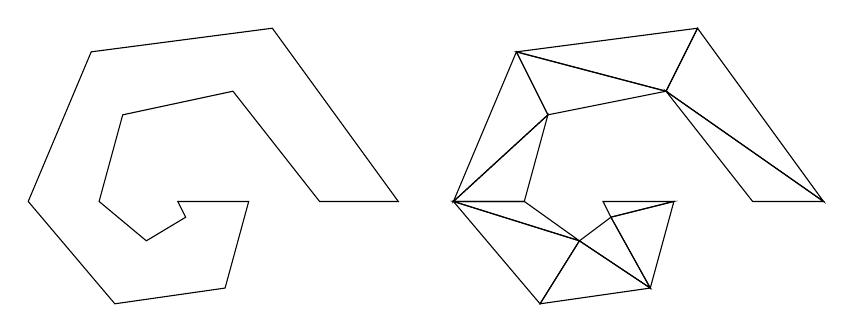
\begin{tikzpicture}
        \draw (1.3, 1.5) -- (1.6, 2.6) -- (3.0, 2.9) -- (4.1, 1.5) -- (5.1, 1.5) -- (3.5, 3.7) -- (1.2, 3.4) -- (0.4, 1.5) -- (1.5, 0.2) -- (2.9, 0.4) -- (3.2, 1.5) -- (2.3, 1.5) -- (2.4, 1.3) -- (1.9, 1.0) -- cycle;

        \pause
        \draw (7.8, 1.3) -- (7.4, 1.0) -- (8.3, 0.4) -- cycle;
        \draw (7.8, 1.3) -- (8.3, 0.4) -- (8.6, 1.5) -- cycle;
        \draw (7.8, 1.3) -- (8.6, 1.5) -- (7.7, 1.5) -- cycle;
        \draw (6.9, 0.2) -- (8.3, 0.4) -- (7.4, 1.0) -- cycle;
        \draw (6.9, 0.2) -- (7.4, 1.0) -- (5.8, 1.5) -- cycle;
        \draw (5.8, 1.5) -- (7.4, 1.0) -- (6.7, 1.5) -- cycle;
        \draw (5.8, 1.5) -- (6.7, 1.5) -- (7.0, 2.6) -- cycle;
        \draw (5.8, 1.5) -- (7.0, 2.6) -- (6.6, 3.4) -- cycle;
        \draw (7.0, 2.6) -- (8.5, 2.9) -- (6.6, 3.4) -- cycle;
        \draw (9.6, 1.5) -- (10.5, 1.5) -- (8.5, 2.9) -- cycle;
        \draw (8.9, 3.7) -- (6.6, 3.4) -- (8.5, 2.9) -- cycle;
        \draw (8.9, 3.7) -- (8.5, 2.9) -- (10.5, 1.5) -- cycle;
      \end{tikzpicture}
      \caption{Podział płaszczyzny na trójkąty}
    \end{figure}
  \end{center}
\end{frame}

\begin{frame}
  \frametitle{Triangulacja w geometrii - przykład trójwymiarowy}
  \begin{center}
    \begin{figure}
      \includegraphics[scale=0.5]{3d-triangulation}
      \caption{Podział bryły na czworościany}
    \end{figure}
  \end{center}
\end{frame}

\begin{frame}
  \frametitle{Triangulacja w teorii grafów}
  \begin{definition}
    Graf planarny to graf, który można narysować na płaszczyźnie w taki sposób, że jego krawędzie nie przecinają się ze sobą.
  \end{definition}

  \begin{example}
    \begin{center}
      \begin{figure}
        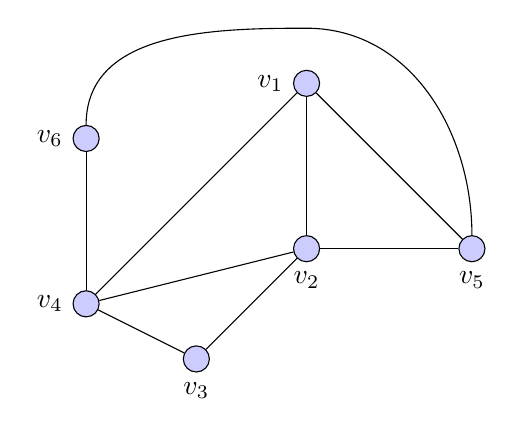
\begin{tikzpicture}[scale=0.7]
          \node[circle, draw, fill=blue!20, label=left:{$v_1$}] (v1) at (2,3) {};
          \node[circle, draw, fill=blue!20, label=below:{$v_2$}] (v2) at (2,0) {};
          \node[circle, draw, fill=blue!20, label=below:{$v_3$}] (v3) at (0,-2) {};
          \node[circle, draw, fill=blue!20, label=left:{$v_4$}] (v4) at (-2,-1) {};
          \node[circle, draw, fill=blue!20, label=below:{$v_5$}] (v5) at (5,0) {};
          \node[circle, draw, fill=blue!20, label=left:{$v_6$}] (v6) at (-2,2) {};

          \coordinate (ctrl-5-6) at (2,4);

          \draw (v1) -- (v2);
          \draw (v1) -- (v5);
          \draw (v2) -- (v3);
          \draw (v2) -- (v4);
          \draw (v2) -- (v5);
          \draw (v3) -- (v4);
          \draw (v4) -- (v1);
          \draw (v4) -- (v6);
          \draw (v5) to[out=90, in=0] (ctrl-5-6) to[out=180, in=90] (v6);
        \end{tikzpicture}
        \caption{Przykład grafu planarnego}
      \end{figure}
    \end{center}
  \end{example}
\end{frame}

\begin{frame}
  \frametitle{Triangulacja w teorii grafów}
  \begin{definition}
    Maksymalny graf planarny to \textbf{graf planarny, do którego nie można dodać żadnej krawędzi bez utraty własności planarnych}. W maksymalnym grafie planarnym każda ściana jest trójkątem (wliczając ścianę zewnętrzną).
  \end{definition}

  \pause
  \begin{definition}
    Triangulacja to \textbf{proces tworzenia grafu maksymalnie planarnego ze zbioru punktów}.
  \end{definition}

  \pause
  \begin{theorem}
    Jeśli maksymalny graf planarny ma $n$ wierzchołków, gdzie $n \geq 3$, to ma dokładnie $3n - 6$ krawędzi i $2n - 4$ ścian. \qed
  \end{theorem}
\end{frame}

\begin{frame}
  \frametitle{Triangulacja w teorii grafów - przykład}
  \begin{center}
    \begin{figure}
      \begin{tikzpicture}[scale=0.5]
        \node[circle, draw, fill=blue!20, label=left:{$v_1$}] (v1) at (0,5) {};
        \node[circle, draw, fill=blue!20, label=right:{$v_2$}] (v2) at (0,0) {};
        \node[circle, draw, fill=blue!20, label=left:{$v_3$}] (v3) at (0,-5) {};
        \node[circle, draw, fill=blue!20, label=above:{$v_4$}] (v4) at (2,2) {};
        \node[circle, draw, fill=blue!20, label=below:{$v_5$}] (v5) at (2,-2) {};
        \node[circle, draw, fill=blue!20, label=right:{$v_6$}] (v6) at (-2,2) {};
        \node[circle, draw, fill=blue!20, label=left:{$v_7$}] (v7) at (-2,-2) {};
        \node[circle, draw, fill=blue!20, label=below:{$v_8$}] (v8) at (-6,0) {};
        \node[circle, draw, fill=blue!20, label=below:{$v_9$}] (v9) at (6,0) {};
        \node[circle, draw, fill=blue!20, label=below:{$v_{10}$}] (v10) at (-9,0) {};
        \node[circle, draw, fill=blue!20, label=below:{$v_{11}$}] (v11) at (9,0) {};

        \coordinate (ctrl-1-3) at (11, 0);

        \pause
        \draw (v1) -- (v6);
        \pause
        \draw (v1) -- (v2);
        \draw (v2) -- (v6);
        \pause
        \draw (v1) to[out=0, in=90] (ctrl-1-3) to[out=-90, in=0] (v3);
        \draw (v1) -- (v4);
        \draw (v1) -- (v8);
        \draw (v1) -- (v9);
        \draw (v1) -- (v10);
        \draw (v1) -- (v11);
        \draw (v2) -- (v3);
        \draw (v2) -- (v4);
        \draw (v2) -- (v5);
        \draw (v2) -- (v7);
        \draw (v2) -- (v8);
        \draw (v2) -- (v9);
        \draw (v3) -- (v5);
        \draw (v3) -- (v7);
        \draw (v3) -- (v8);
        \draw (v3) -- (v9);
        \draw (v3) -- (v10);
        \draw (v3) -- (v11);
        \draw (v4) -- (v9);
        \draw (v5) -- (v9);
        \draw (v6) -- (v8);
        \draw (v7) -- (v8);
        \draw (v8) -- (v10);
        \draw (v9) -- (v11);

        \pause
        \draw[fill=blue!30, draw=black] (0,5) -- (0,0) -- (-2,2) -- cycle;
        \node[fill=white] at (0,-2) {Wszystkie ściany są trójkątami (także zewnętrzna)};
      \end{tikzpicture}
      \caption{Graf Goldnera-Harary'ego - przykład grafu maksymalnie planarnego o 11 wierzchołkach i 27 krawędziach}
    \end{figure}
  \end{center}
\end{frame}

\begin{frame}
  \frametitle{Triangulacja w teorii grafów}
  \begin{definition}
    Cykl indukowany to taki cykl w grafie, że żadne dwa jego wierzchołki nie są połączone krawędzią, która nie należy do cyklu.
  \end{definition}

  \begin{definition}
    Graf cięciwowy to graf, w którym każdy \textbf{cykl o długości czterech lub większej ma przekątną}, czyli krawędź łączącą dwa niekolejne wierzchołki cyklu.

    W grafie takim cykle indukowane mają zawsze długość 3.
  \end{definition}
  \pause
  \begin{definition}
    Triangulacja to proces dodawania krawędzi do grafu w celu \textbf{otrzymania grafu cięciwowego}.
  \end{definition}
\end{frame}

\begin{frame}
  \frametitle{Triangulacja w teorii grafów - przykład}
  \begin{center}
    \begin{figure}
      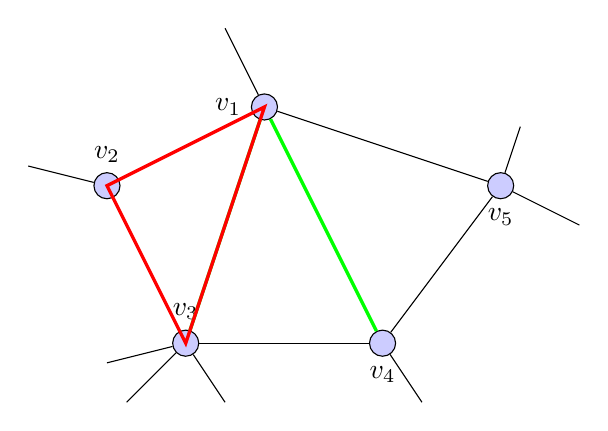
\begin{tikzpicture}[scale=1.0]
        \node[circle, draw, fill=blue!20, label=left:{$v_1$}] (v1) at (0,1) {};
        \node[circle, draw, fill=blue!20, label=above:{$v_2$}] (v2) at (-2,0) {};
        \node[circle, draw, fill=blue!20, label=above:{$v_3$}] (v3) at (-1,-2) {};
        \node[circle, draw, fill=blue!20, label=below:{$v_4$}] (v4) at (1.5,-2) {};
        \node[circle, draw, fill=blue!20, label=below:{$v_5$}] (v5) at (3,0) {};

        \draw (v1) -- (-0.5, 2);
        \draw (v1) -- (v2);
        \draw (v2) -- (-3, 0.25);
        \draw (v2) -- (v3);
        \draw (v3) -- (-2, -2.25);
        \draw (v3) -- (-1.75, -2.75);
        \draw (v3)-- (-0.5, -2.75);
        \draw (v3) -- (v4);
        \draw (v4) -- (2, -2.75);
        \draw (v4) -- (v5);
        \draw (v5) -- (4, -0.5);
        \draw (v5) -- (3.25, 0.75);
        \draw (v5) -- (v1);

        \pause
        \draw[very thick, color=green] (v1) -- (v3);
        \draw[very thick, color=green] (v1) -- (v4);

        \pause
        \draw[very thick, draw=red] (0,1) -- (-2,0) -- (-1,-2) -- cycle;

      \end{tikzpicture}
      \caption{Przykład triangulacji grafu poprzez dodanie krawędzi $(v_1, v_3)$ oraz $(v_1, v_4)$. W procesie tym powstały trzy cykle indukowane o długości 3.}
    \end{figure}
  \end{center}
\end{frame}

\begin{frame}
  \frametitle{Źródła}
  \begin{thebibliography}{6}
    \bibitem{1} \url{https://mathworld.wolfram.com/Triangulation.html}
    \bibitem{2} \url{https://en.wikipedia.org/wiki/Triangulation_(disambiguation)}
    \bibitem{3} \url{https://en.wikipedia.org/wiki/Planar_graph\#Maximal_planar_graphs}
    \bibitem{4} \url{https://en.wikipedia.org/wiki/Chordal_graph}
    \bibitem{5} \url{https://en.wikipedia.org/wiki/Simplex}
    \bibitem{6} \url{https://facultyweb.kennesaw.edu/mlavrov/courses/graph-theory/lecture21.pdf}
  \end{thebibliography}
\end{frame}

\end{document}
